\begin{figure}[t]
  \centering
  \vspace{2mm}
  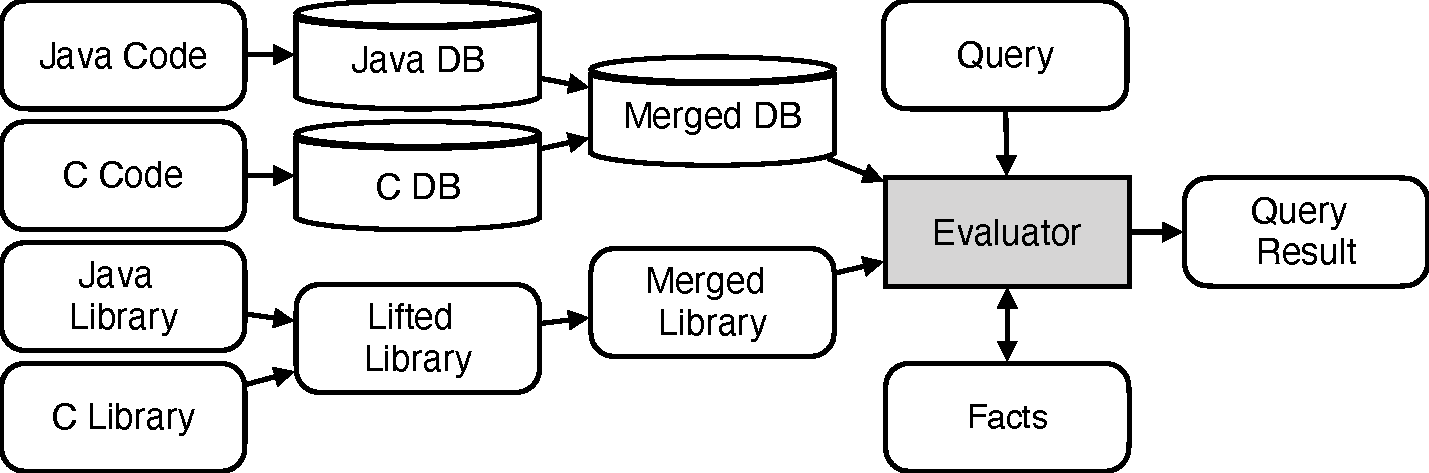
\includegraphics[width=0.7\textwidth]{img/codeql.pdf}
  \caption{Overall structure of \ours for JNI programs}
  \label{fig:codeql}
\end{figure}

%\section{Implementation}\label{sec:impl}
\section{\ours: Extension of CodeQL for multilingual program analysis}\label{sec:impl}
In this section, we present \ours, a prototype extension of
CodeQL~\cite{codeql} for multilingual program analysis.  \ours tracks
dataflows across language boundaries in two types of multilingual programs:
1) Java-C programs interoperating via Java Native Interface(JNI)~\cite{jnispec} and
2) Python-C programs interoperating via Python Extension Module~\cite{pyext}.
For simplicity, we use the Java-C program analysis to explain the common
parts and emphasize the Python-C program analysis in Section~\ref{sec:merging2}.

%In this section, we present \ours, a prototype implementation of our
%approach of extending declarative static analysis for multilingual programs,
%in the case of dataflow analysis for JNI programs(Java-C)
%and extension module programs(Python-C) using CodeQL~\cite{codeql}.
%Dataflow analysis is an analysis to determine if a value that is created at
%certain program location, source, can flow into another certain program location, sink.
%Without loss of generality, we will mainly explain analysis of JNI program
%analysis throughout most of the section, since the difference between JNI programs and
%extension module programs is relevent only when defining
%language-interoperation rules.



\subsection{CodeQL}
%CodeQL is a static analysis engine that transforms source code programs into
%databases, and performs analysis by evaluating queries written in the
%declarative and object-oriented language called QL (Query Language).
%In QL, there are mainly two syntax for defining rules.
%They are defining ``predicates'' or ``classes.''
%The following QL code defines the predicate \codeql{isOneOrTwo}:

CodeQL is a declarative static analysis engine that transforms source code into
a database of facts and performs analyses by evaluating queries written in the
declarative and object-oriented language called QL (Query Language). Using QL,
one can depict rules by defining ``predicates'' and ``classes.'' The following
QL code defines the unary predicate \codeql{isOneOrTwo}:

\begin{lstlisting}[style=codeql,xleftmargin=2.5em]
predicate isOneOrTwo(int n) {
  n = 1 or n = 2
}
\end{lstlisting}

\noindent
which states that the fact \codeql{isOneOrTwo(n)} is derivable from either one
of the two facts, \codeql{n = 1} and \codeql{n = 2}.
Some predicates may have a return type and a special variable named {\tt
result}, as the following predicate \codeql{addOne}:

\begin{lstlisting}[style=codeql,xleftmargin=2.5em]
int addOne(int n) {
  isOneOrTwo(n) and result = n + 1
}
\end{lstlisting}
\noindent
The predicate is syntactic sugar equivalent to the following ordinary predicate:
%For example,
%\codeql{addOne} can be rewritten as the following binary predicate \codeql{addOnePred}:
%
\begin{lstlisting}[style=codeql,xleftmargin=2.5em]
predicate addOnePred(int n, int result) {
  isOneOrTwo(n) and result = n + 1 
}
\end{lstlisting}
\noindent
An equality formula \codeql{m = addOne(n)} is also syntactic sugar equivalent
to \codeql{addOnePred(n, m)}.
%\inred {
%and the formula \codeql{m = addOne(n)} is equivalent to \codeql{addOnePred(n, m)}
%}

In QL, defining classes is one way to define user-defined types. 
The following QL code defines a class named \codeql{OneOrTwo}:
\begin{lstlisting}[style=codeql,xleftmargin=2.5em]
class OneOrTwo extends int {
  // characteristic predicate
  OneOrTwo() { this = 1 or this = 2 }
  // member predicate
  int add(OneOrTwo that) { result = this + that }
}
\end{lstlisting}
\noindent
The class extends {\tt int}, which means that the class is a subtype of {\tt
int}.
Unlike other object-oriented languages, QL classes cannot be instantiated.
Instead, a class defines a special predicate, called {\it characteristic
predicate}, that has the same name to the class, and all values satisfying the
predicate are deemed elements of the class.
%A class defines a set of elements that satisfy the predicate called
%``characteristic predicate.'' 
For example, only two integer values, {\tt 1} and {\tt 2}, are elements of the
class \codeql{OneOrTwo}, because its characteristic predicate is satisfied only
when {\tt this} is {\tt 1} or {\tt 2}.
A class can also have {\it member predicates} that relate itself with other
values.
Member predicates are also syntactic sugar of ordinary predicates. 
For example, the member predicate \codeql{add} is equivalent to the following
ternary predicate: 
\begin{lstlisting}[style=codeql,xleftmargin=2.5em]
predicate addPred(OneOrTwo this, OneOrTwo that, int result) {
  result = this + that
}
\end{lstlisting}
Thus, an equality formula \codeql{z = x.add(y)} is equivalent to
\codeql{addPred(x, y, z)}.
For more detailed information about CodeQL, refer to the paper of Avgustinov et
al.\cite{ql2016} or the official document~\cite{codeql}.

%Figure~\ref{fig:codeql} presents the overall structure of \ours for JNI programs.
%First, it generates databases for both languages, C\footnote{
%Even though \ours analyzes JNI programs written in Java and both C and
%C++, this paper refers to C only fore presentation brevity.} and
%Java, and merges them to one database.  This corresponds
%to the step of extracting syntactic datafacts from source code programs.
%Then, we merge the common datafacts and rules in both languages,
%which are parts of their libraries that CodeQL provides, into one merged library.
%Finally, using the merged database and merged library, a user can write a query to
%perform a client-analysis, and evaluate it to produce its analysis result.

Figure~\ref{fig:codeql} presents the overall structure of \ours for JNI
programs.  First, it generates databases for both languages, C\footnote{ Even
though \ours analyzes JNI programs written in Java and both C and C++, this
paper refers to C only for presentation brevity.} and Java, and merges them into
one database.  This corresponds to the step of extracting the initial syntactic
facts from the source code.  Then, \ours~merges the common rules in both
languages, which are parts of their libraries that CodeQL provides, into one
merged library.  Finally, using the merged database and merged library, a user
can write a query to perform a client-analysis and evaluate it to produce its
analysis result.

\subsection{Creating Databases}
For compiled languages such as C and Java, CodeQL generates their databases by
compiling source programs.  When a compiler compiles a program, CodeQL monitors
the compiler to extract necessary information and creates a database with the
extracted information. For scripting languages like Python, CodeQL uses its own
extractor to directly extract necessary information from source code.
CodeQL creates a database for a single language in two steps:
1) it stores the extracted information in a \textit{trap} file, a human
readable format file for the CodeQL database, and 2) it transforms the trap
file into a database in the binary format. 
For example, the following demonstrates a sample trap file:

\begin{lstlisting}[style=java,numbers=none]
#10001=@"class;myClass.MyClass"
#10002=@"type;int"
primitives(#10002,"int")
#10003=@"callable;{#10001}.myMethod({#10002}){#10002}"
#10004=@"params;{#10003};0"
params(#10004,#10002,0,#10003,#10004)
paramName(#10004,"myParam")
...
\end{lstlisting}

\noindent
which describes the parameter information of the method \javacode{myMethod}.
It also shows facts that will eventually be stored in tables:
\javacode{primitives(...)}, \javacode{params(...)}, and
\javacode{paramName(...)}.
The database manages tables based on fact types. For example, it stores
the fact \javacode{primitives(...)} in a table named \javacode{@primitives}, and
\javacode{params(...)} in a different table named \javacode{@params}.

%Here, each line of \javacode{primitives(...)},
%\javacode{params(...)}, and
%\javacode{paramName(...)}
%corresponds to one fact, which will be
%finally stored in each table of database.

To create a single merged database for both C and Java, \ours maintains a
separate trap file for each language and then merges them into a trap file.
One problem is that the mergence fails due to the name collision if a table
with the same name exists in both trap files.
To avoid the problem, \ours renames each table to a globally unique name, by
appending a language-specific prefix to the table name before the mergence.
For example, if a table named \codeql{@params} exists in both C and Java trap
files, \ours renames the table in C to \codeql{@c\_params} and the table in
Java to \codeql{@java\_params}.
After renaming such tables, \ours merges the trap files into a database on
which predicates and queries are evaluated.

%To create a single database for both C and Java, \ours maintains
%a separate trap file for each language and then merges them.
%Note that both trap files may have tables with the same name.
%To avoid name conflicts in a merged database, we add a
%language-specific prefix to each table.
%For example, if both trap files have tables named \codeql{@params},
%we rename the table from C as \codeql{@c\_params},
%and the table from Java as \codeql{@java\_params"}.
%After renaming such tables, we can safely finalize the trap files into
%databases on which queries can be evaluated.

\subsection{Lifting Libraries}

CodeQL provides various libraries for C and Java, including
pre-defined predicates and classes for users to implement their own analyses.
A dataflow analysis library is such a library, which supports both C and Java.
For example, Figure~\ref{fig:qll} (a) and (b) show sample QL libraries for C
and Java respectively, which use the same class name \ccode{Node} and the same
predicate name \ccode{localFlowStep}.
However, even with the same name, the class \ccode{Node} in C and the
class \javacode{Node} in Java are different classes, which are incompatible.
The same applies to the predicate \ccode{localFlowStep}.
In other words, we can not use the class \ccode{Node} in C as an
argument of the predicate \javacode{localFlowStep} in Java or vice versa.

\begin{figure}[hbt!]
  \centering
%  \vspace{2mm}
  \begin{subfigure}{0.94\textwidth}
\begin{lstlisting}[style=codeql,xleftmargin=2.5em]
class Node { ... }

predicate localFlowStep(Node from, Node to) {
  // Expr -> Expr
  exprToExprStep_nocfg(from.asExpr(), to.asExpr())
  or
  // Assignment -> LValue post-update node
  ...
}
\end{lstlisting}
    \vspace*{-.5em}
    \caption{\normalsize c/dataflow/internal/DataFlowUtil.qll}
    \label{fig:qll1}
  \end{subfigure}
  \begin{subfigure}{0.94\textwidth}
\begin{lstlisting}[style=codeql,xleftmargin=2.5em]
class Node { ... }

predicate localFlowStep(Node node1, Node node2) {
  // Variable flow steps through assignment expression
  node2.asExpr().(AssignExpr).getSource() = node1.asExpr()
  or
  // Variable flow steps through adjacent def-use and use-use pairs.
  ...
}
\end{lstlisting}
    \vspace*{-.5em}
    \caption{\normalsize java/dataflow/internal/DataFlowUtil.qll}
    \label{fig:qll2}
  \end{subfigure}
  \begin{subfigure}{0.94\textwidth}
\begin{lstlisting}[style=codeql,xleftmargin=2.5em]
module C { /* original classes and predicates from C lib */ }
module JAVA { /* original classes and predicates from Java lib */ }

private newtype TNode =
  TJavaNode(JAVA::Node n)
  or
  TCNode(C::Node n)
class Node extends TNode {
  JAVA::Node asJavaNode() { this = TJavaNode(result)}
  C::Node asCNode() { this = TCNode(result) } ...
}

predicate localFlowStep(Node node1, Node node2) {
  JAVA::localFlowStep(node1.asJavaNode(), node2.asJavaNode())
  or
  C::localFlowStep(node1.asCNode(), node2.asCNode())
}
\end{lstlisting}
    \vspace*{-.5em}
    \caption{\normalsize jni/dataflow/internal/DataFlowUtil.qll}
    \label{fig:qll3}
  \end{subfigure}
  \vspace*{-.5em}
  \caption{QL libraries for C and Java}
  \label{fig:qll}
\end{figure}

To make classes and predicates in C and Java compatible,
\ours lifts each library to the common level.
First, as on lines 1 and 2 of Figure~\ref{fig:qll3}, \ours encapsulates the
original dataflow libraries for C and Java in separate modules named {\tt C}
and {\tt Java},
respectively.\footnote{https://codeql.github.com/docs/ql-language-reference/modules/}
After the encapsulation, the original classes and predicates can be referenced
via the module containing them. 
%The encapsulation prevents the name collision between the original Java and C
%libraries as well as between the original libraries and lifted ones \ours
%defines.
%\ours encapsulate each of the original dataflow libraries with a CodeQL
%module system\footnote{https://codeql.github.com/docs/ql-language-reference/modules/}
%and name each of them \codeql{C} and \codeql{JAVA} so that it can distinguish the original
%classes and predicates by lifted ones. 
For example, \codeql{Java::Node} refers to the original class \codeql{Node} in
the module {\tt Java}.
Lines from 4 to 11 of Figure~\ref{fig:qll3} demonstrate the lifted class of the
original class {\tt Node}.
\ours lifts a class by first defining a sum
type\footnote{https://codeql.github.com/docs/ql-language-reference/types/\#algebraic-datatypes},
denoting that the lifted class comes either from C or Java, and then making the
lifted class be of that type.  
The lifted class defines two member predicates, \codeql{asCNode} and
\codeql{asJavaNode}, that downcasts elements of the lifted class into elements
of the original C or Java class.
Lines from 13 to 17 of Figure~\ref{fig:qll3} demonstrate the lifted predicate
of the original predicate {\tt localFlowStep}.
Similarly, \ours lifts a predicate by combining two original predicates with
the \codeql{or} connective. For each predicate, arguments and return values are
downcasted to elements of the class of their corresponding language.
After lifting, lifted predicates show the equivalent behaviors as the original
ones if all the arguments are from the same language.

\ours can fully automate the lifting process using QL compiler error
messages. When compiling a query without importing the library, the QL compiler
reports error messages containing required classes and predicates, and
signatures of the predicates. Using the information, \ours
automatically synthesizes lifted classes and predicates.

%The process of lifting could be effectively automated with the aid of
%QL's compile message. First, try to compile a query without actually
%importing the library, then the QL compiler will give error message
%that contains all the iinformation about required yet missing predicates and classes,
%such as name, arity or signature of each predicate. Using this information,
%the lifted predicates and classes can be automatically synthesized, without
%manually searching for what are the required ones.

\subsection{Merging Libraries: Java-C}\label{sec:merging}
After lifting libraries for different languages, we manually extend predicates
to reflect the interoperation semantics between multiple languages.  
For the Java-C program analysis, we identified various interactions from Java
to C and vice versa via JNI, and extended predicates to model their
behaviors.
%
%After lifting libraries for different languages, we extend predicates to
%reflect the interoperation semantics between multiple languages.
%For analyzer for JNI programs, We identified various interactions from Java to C and from C to Java
%and extended predicates to model their behaviors.
%
For example, the following shows how we extend the predicate
named \codeql{viableCallable}:
\begin{lstlisting}[style=codeql,xleftmargin=2.5em]
DataFlowCallable viableCallable(DataFlowCall c) {
  result.asJavaNode()    = JAVA::viableCallable(c.asJavaNode())
  or result.asCNode()    = C::viableCallable(c.asCNode())
  or result.asCNode()    = viableCallableJ2C(c.asJavaNode())
  or result.asJavaNode() = viableCallableC2J(c.asCNode())
}
\end{lstlisting}
%This predicate finds the call edge from the call expression to its
%target, and is required for finding data flows through the fnction arguments and returns.

\noindent
It finds call edges from call expressions to their targets. 
Lines 2 and 3 show the results of lifting using
original predicates from the dataflow libraries.  
They handle intra-language call edges from Java to Java and from C to C, respectively.
Lines 4 and 5 show the results of merging libraries, representing
inter-language call edges.  The predicate \codeql{viableCallableJ2C} finds call edges
from Java to C, and \codeql{viableCallableC2J} finds call edges from C to Java.
%Because these two call edges have different characteristics, we
%implemented them differently.

%\medskip
\textbf{Java to C.} In Java-C programs, one can make interactions from Java to
C by calling native functions in C from Java code. 
The target of such a function call is determined in a static manner.
The target function should follow the JNI naming convention, which is adding
\codeql{Java\_} as prefix, followed by a fully qualified name of its class and
the additional \codeql{\_}, to the method name.
For example, the target function name for a function call of \codeql{cfunction}
would be \codeql{Java\_fully\_qualified\_class\_name\_cfunction}.
With this convention, we can define \codeql{viableCallableJ2C} so that
\codeql{f = viableCallableJ2C(call)} holds when \codeql{f.toString() = "Java\_"
+ call.getTarget().className() + "\_" +} \\
\codeql{call.getTarget().getName()} holds.


%\smallskip
\textbf{C to Java.} The interaction from C to Java is more complex and
requires more careful implementation than the interaction from Java to C.
The primary difference is that a method call from C to Java requires
the runtime values of variables, which may not be always possible.
First, C code calls the interface function \ccode{GetMethodID(name, sig)}
to get the ``method ID'' of the Java method whose name matches the first argument
and the type signature matches the second argument passed to this function.
This method ID is stored at a variable, say \ccode{mid}, and
an actual method call is invoked by another
interface function, \ccode{Call<type>Method(obj, mid, args...)}. Calling this interface 
function corresponds to calling the method that \ccode{mid} indicates
with \ccode{obj} as ``this object'' and \ccode{args} as the arguments.

To correctly handle this method call, we should be able to answer these
questions: ``When we call \ccode{GetMethodID},
what are the string values of \ccode{name} and \ccode{sig}?'' and
``When we call \ccode{Call<type>Method}, what is the method ID value of \ccode{mid}?''
Soundly answering these questions requires inter-language dataflow analysis
because the string or method ID values may be passed across language boundaries.
However, we observed that such a pattern rarely happens in practice,
and using only intra-language dataflow analysis within C code is enough for most cases.
Therefore, we decided to sacrifice the precision
by using intra-language analysis instead of inter-language analysis
as a trade-off for a more lightweight and simpler implementation.
We implemented two intra-flow analysis modules for C,
which find 1) dataflows from string literals to the arguments of interface functions
and 2) dataflows from interface function call results to the arguments of interface functions.
Using these modules, we can implement the
predicate \codeql{viableCallableC2J} by adding a call edge from a \ccode{Call<type>Method}
call to the method \ccode{m}, if there is a flow to \ccode{mid} from a
call to \ccode{GetMethodID}, and string values that flow into the
arguments \ccode{name} and \ccode{sig} of \ccode{GetMethodID} that
correspond to the name and the type signature of the method \ccode{m}.

In addition to the predicate \codeql{viableCallable},
we extended more predicates to consider other JNI interface functions such as
\ccode{findClass} and \ccode{GetFieldID}.
Most of such extended predicates are specialized \codeql{step} predicates.
We extended them in a similar way to the calls from C to Java described above.

\subsection{Merging Libraries: Python-C}\label{sec:merging2}
%The extension module programs requires its own modelling for its own interoperation
%semantics to be analyzed.
%The following is the extension of the predicate \codeql{viableCallable}
%for extension module programs:

To analyze Python-C programs, we extended predicates to model the
interoperation semantics of Python Extension Module.
The following shows \codeql{viableCallable} predicate we extended for the
Python-C program analysis: 

\begin{lstlisting}[style=codeql,xleftmargin=-.5em,numbers=none]
DataFlowCallable viableCallable(DataFlowCall c) {
  result.asPythonNode()    = PYTHON::viableCallable(c.asPythonNode())
  or result.asCNode()      = C::viableCallable(c.asCNode())
  or result.asCNode()      = viableCallableP2C(c.asPythonNode())
  or result.asPythonNode() = viableCallableC2P(c.asCNode())
}
\end{lstlisting}

\noindent
The only different parts from the Java-C program analysis are the predicates
\codeql{viableCallableP2C} and \codeql{viableCallableC2P}.

%Again, line 2 and line 4 are direct outcomes of the process of lifting,
%and all we have to newly define is the language-interoperation predicates,
%\codeql{viableCallableP2C} and \codeql{viableCallableC2P}. 

\textbf{Python to C.} Similar to the interactions from Java to C, one can make
interactions from Python to C by importing and calling functions from
C. Python Extension Module provides a pre-defined C struct \ccode{PyMethodDef} to
export a C function to Python: 
%Similar to JNI programs,
%in python program with 
%extension modules, one can make interactions from
%Python to C by importing and calling C functions that are exported via
%extension modules. There is a C structure "PyMethodDef"
%that stores the information about the c function that is exported. If we define
%the structure

\begin{lstlisting}[style=mcpp]
struct PyMethodDef methods[] = {
  {
    .ml_name = "cfunction",
    .ml_meth = cfunction_impl, ...
  }, ...
}
\end{lstlisting}

\noindent
The member field \ccode{ml_name} has a visible name of a C function to Python,
and the member field \ccode{ml_meth} has the pointer to the actual C function.
Thus, the function \ccode{cfunction_impl} defined in C code is invoked when
importing and calling \ccode{cfunction} in Python code.
To model the behavior, we define the CodeQL class \codeql{PyMethodDef}
and the predicate \codeql{viableCallableP2C}. The class \codeql{PyMethodDef}
corresponds to the C structure \ccode{PyMethodDef}. It has
two member predicates \codeql{getName()} and \codeql{getFunc()} whose results are
the values of the fields \ccode{ml_name} and \ccode{ml_meth}, respectively.
Then, we make a rule for \codeql{viableCallableP2C} such that for some \codeql{def} of type \codeql{PyMethodDef},
if \codeql{def.getName() } \codeql{= call.getTarget().toString()}
for some \codeql{call}, then \codeql{def.getFunc() } \codeql{= viableCallableP2C(call)} holds.


% Then, we define
% \codeql{f = viableCallableP2C(call)} holds when there exists \codeql{def}
% of type \codeql{PyMethodDef} such that \codeql{f = def.getFunc()} and
% \codeql{call.getTarget().toString()} \codeql{= def.getName()} holds.

In addition, we define rules that connect dataflows from arguments of
a Python-to-C function call to parameters of its target C function.
Unlike the Java-to-C function call semantics, Python Extension Module
packs arguments in a Python tuple object and propagates the object to a single
parameter of the target C function. 
Then, the target C function unpacks the tuple object into individual Python
objects by calling the \ccode{PyArg_ParseTuple} API. 
This means that the usual way of connecting arguments and parameters via their
positions does not work, and we need another way.
We modelled this behavior by defining \codeql{VirtualArgNode}, a subclass of \codeql{Node},
that corresponds to the Python tuple object. Then, we define some predicates
for representing flows in and out of this node. First, we define a
step that represents the flow from values of original argument nodes to virtual argument nodes. We then define
a step that represents the flow from the values of virtual argument nodes to a single parameter node in a C function.
By doing so, the flows from original argument nodes to use sites will be
found in three steps: 1) from an argument node to a virtual argument node,
2) from the virtual argument node to the parameter node of a C function,
and 3) from the parameter node to the out node of \ccode{PyArg_ParseTuple} API function call.


%then the Python code can import cfunction and the call expression cfunction()
%will resolve to the actual function cfunction\_impl defined in C code. To model
%this behavior, we can define \codeql{viableCallableP2C} so that \codeql{f =
%viablaCallableP2C(call)} holds when \codeql{f = def.getFunc()} and
%\codeql{call.getTarget().toString() = def.getName()} holds.

\medskip
%\textbf{C to Python.} The interaction from C to Python also requires
%the runtime values of variables, which makes the analysis a bit complex. 
%C code calls the interface function \ccode{PyObject\_CallObject(func, args)}
%where func is the python function object, and the args is the python tuple
%object. Finding call target of this API function call simply reduces to answering the
%question: ``what is the value of \ccode{func}?'' Again, we define
%``intra-flows'' for both Python and C to answer this question efficiently: 1) dataflows from 
%python function any to arguments in Python and 2) dataflow from any parameters to the first argument of
%\ccode{PyObject\_CallObject} in C. Then, the value that \ccode{func} may have
%is found via three big steps: finding flow from Python function to an argument, from the argument to
%a c parameter, and from the parameter to the variable \ccode{func}.

\textbf{C to Python.} The interaction from C to Python requires the runtime
values of variables, similar to the interaction from C to Java. 
To invoke Python functions in C, C code calls the interface function
\ccode{PyObject_CallObject(func, args)}, where \ccode{func} is a Python
function object, and \ccode{args} is a Python tuple object that contains
all arguments. 
Because C code can get Python objects as
function arguments of the Python-to-C function calls,
we define two
``intra-flows'' analyses to identify Python objects assigned to \ccode{func}:
1) dataflows from a Python function object to the argument of a C function call,
and 2) dataflows from the parameters of a C function to the first argument of \ccode{PyObject_CallObject}.
Using these intra-flow analyses, we can find actual targets that should be invoked
for \ccode{PyObject_CallObject} API function calls.


%\textbf{Args and Params.} After finding the call target of the given call
%expression, Then we have to connect the dataflow from the arguments to
%aprameters.  This is tirivial for JNI programs, but in case of extension module
%programs, it requires a bit of effort. When you call a c function from the
%Python code with arguments, then all the arguments are implicitly packed in a
%tuple, and that tuple is passed to c function as a single argument. Then the
%writter of c function should manually call API function,
%\ccode{PyArg\_ParseTuple} to unpack this tuple to get each individual
%arguments. This behavior is modelled by creating virtual argument node which is
%a virtual Python tuple object, and create the store step from the real argument
%to the virtual argument.  By doing so. the real argument will flow to the real
%use site of in three steps: 1) store step from the argument to virtual
%argument, 2) function-in step from virtual argument to the parameter of target
%C function, and 3) read step from the parameter to its tuple-read API fuction.
%The similar thing happens when there is a call from C to Python. The actual
%argument of C API function is a tuple object, but this tuple is implicitly
%unpacked and each element is assigned to each parameter of Python method.
%Again, the solution is to create virtual parameter in Python, and create the
%read step from the virtual tuple parameter to actual parameters.
